\subsubsection*{NRM}

\paragraph{Overview}

Argo Node Resource Manager (NRM) is a daemon running on the compute
nodes. It centralizes node management activities such as local application
launching, resource management, and power management.

NRM interacts with both global resource management services (e.g., job
scheduler) and with application components and runtime services running on
the node. It acts as a control infrastructure to enable custom resource
management policies at the node level.  Applications can influence these
mechanisms, both directly (through explicit API calls used, e.g., to
request additional resources on the node) and indirectly (by having their
run-time behavior monitored by NRM).

\paragraph{Key Challenges}

Many ECP applications have a complex runtime structure, ranging from in
situ data analysis, through an ensemble of largely independent individual
subjobs, to arbitrarily complex workflow structures.  At the same time, HPC
hardware complexity increases as well, from deeper memory hierarchies to
heterogeneous compute resources and performance fluctuating based on
power/thermal constraints.

Even in the common case of each compute node being allocated exclusively to
a single job, managing available node resources can be a challenge.  If a
compute node is shared among multiple job components (a likely scenario
considering the reduced cost of data transfers), these components---if
allowed to freely share node resources---could interfere with one another,
resulting in suboptimal performance.  It is the NRM's job to rein in this
complexity by acting as a coarse-grained resource arbitrator.

\paragraph{Solution Strategy}

NRM uses an active approach to resource management. Physical and logical
resources on the compute nodes are configured, discovered, and accounted for.
NRM can manage compute nodes and individual components of parallel workloads,
in the sense that it performs an active accounting of two types of interfaces
for those workloads: sensors and actuators. These abstracted components are
available through an upstream API which enables their discovery and management.

The NRM daemon supports power actuators, as well as` sensors based on CPU counters
and power information. We also provide a simple API that application processes
can use to periodically update the NRM on their progress. This gives NRM
reliable feedback on the efficacy of its power policies, and it can also
be used for a more robust identification of the critical path, rather than
relying on heuristics based on performance counters.

\begin{wrapfigure}[12]{r}{.58\textwidth}
  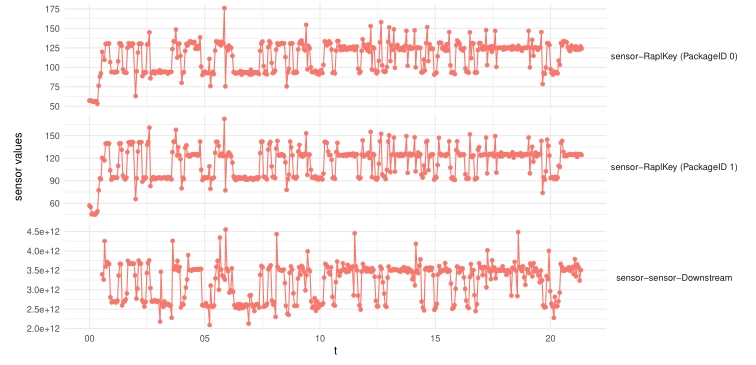
\includegraphics[width=.58\textwidth]{projects/2.3.1-PMR/2.3.1.19-Argo-PowerSteering/sensors}
\end{wrapfigure}
In addition to those capabilities, NRM's configuration format allows for
the configuration of actuators and active polling sensors based on arbitrary
executables. The figure on the right shows a reading of NRM's sensor
outputs for two RAPL sensors along with CPU counter instrumentation. In order
to provide these capabilities, the NRM daemon manages the launching, management,
and stopping of parallel workloads through a unified interface. Resources
can be dynamically reconfigured at run time; these interfaces are provided
for use from applications and from global services.

\begin{wrapfigure}[10]{l}{.38\textwidth}
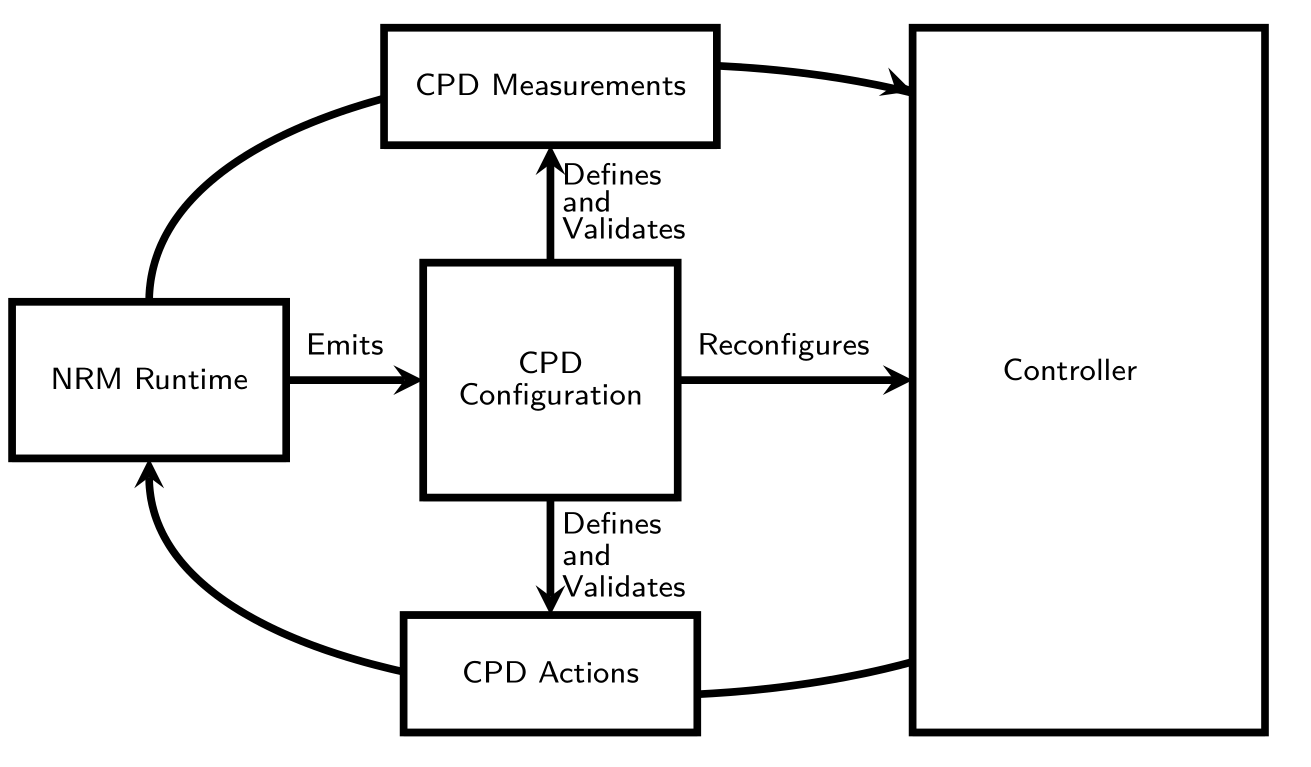
\includegraphics[width=.38\textwidth]{projects/2.3.1-PMR/2.3.1.19-Argo-PowerSteering/cpd}
\end{wrapfigure}
Other than sensor and actuator accounting capabilities, NRM provides
optional support for autonomic node management. This support is provided through
the accounting of node-local autonomic goals and constraints, which are
expressed in terms of available nodes and sensors. These goals and
constraints can be inspected by the users, global services (GRM), and
applications through NRM's unified interface. Inspection is achieved through
the emission of a Control Problem Description (CPD), which outlines active
sensors, actuators, goals, and constraints. This scheme is outlined in the
figure on the left.

\paragraph{Recent Progress}

The NRM daemon has undergone major improvements. In order to improve the
software quality and overall reliability of NRM, the core business logic
of the NRM daemon has been externalized in a shared library, written in the
statically typed language Haskell. This NRM version is pending an upcoming
release. Our custom CI pipeline also has been improved, with the addition
of unit tests and enrichment of existing functional tests. We are still in
the process of leveraging ECP testing infrastructure.

NRM has recently added support for multi-armed bandit based control policies.
In order to make this work as robust as possible, it has been
compartmentalized into a software library (\textit{hbandit}). \textit{hbandit}
implements statically typed, independently tested versions of the relevant
machine learning algorithms.

NRM now offers a Python support library for upstream control. This library is
intended for workload-specific control algorithm experiments.

We continue supporting the \texttt{libnrm} C library that can be linked to
applications in order to provide reports on application progress to NRM. We have
instrumentation for EXAALT, QMCPACK, ExaSMR, AMG, Stream, and CANDLE.
This capability gives us insight into the effect of our resource management
policies on the run-time behavior of user codes.

\paragraph{Next Steps}

We are working on a report to showcase the use of NRM's current autonomic
resource management strategies in the context of workload energy minimization,
through the use of RAPL control and application feedback.

We are also working on expanding the set of ECP applications that are
instrumented to report their progress to NRM, as well as validation of the
infrastructure on multiple ECP platforms.

We are planning to expand the list of resources managed by NRM by
adding support for other vendor-specific mechanisms, as well as better
integration with other ECP system software (job schedulers, application
tracing, and power interfaces).
